\chapter{Background}
\label{background}

\section{Domain-Specific Languages}
Domain-specific languages (DSLs) are, in general, programming languages which have specialized
constructs limited to a specific type of computation. A typical goal of
most domain-specific languages is to improve productivity in a particular domain
by increasing abstraction at the cost of generality. Unlike general-purpose languages like C and Java,
the number of operations and types of data structures in a domain-specific language
are generally limited. The benefit of this is that the language's compiler is
generally aware of each of these operations and able to specialize and optimize them.
Some domain-specific languages are standalone, including a full compiler with standard language
lexing, parsing, and type checking. Others are embedded in a host general purpose language,
leveraging the existing language's compiler infrastructure while also
providing additional specialization or functionality. The semantics of the embedded language
define how code written in the host language and DSL interact.

For example, SQL is a standalone, declarative
domain-specific language originally created in 1986 for describing database operations with high level constructs
for defining operations on tables of data, but little support for other types of operations.
Compilers for SQL include query-planning optimizations which optimize the order of
operations based on domain-specific knowledge about each operator.
Similarly, Halide~\cite{pldi13halide} is an imperative language embedded in C++ specialized for image processing
and operations on arrays. Halide's syntax and compiler are specialized for linear and stenciled access patterns,
as these are extremely common in operations on images.

With the recent explosion of academic and industry interest in the machine learning (ML) domain,
a variety of ML-specific languages have been developed.
OptiML~\cite{optiml} is a mixed (imperative and functional) paradigm DSL embedded in Scala
which specializes in data-parallel operations on vectors and matrices.
Its operator abstractions allow it to automatically parallelize ML applications.
More recently, TensorFlow ~\cite{tensorflow} and PyTorch ~\cite{pytorch} are
embedded DSLs in Python for defining machine learning computation graphs based on
a limited set of operations on multi-dimensional arrays (``tensors''). Both include
notions of auto-gradient computation, making the computation required to
train described graphs essentially implicit.

In this work, we will look specifically at domain-specific languages in the domains under
data analytics, with a particular focus on image processing and machine learning.
We assume here that the target DSLs create an intermediate representation of the program
which can be lowered to another form prior to execution.


\section{Parallel Patterns}

Parallel patterns like \emph{Map}, \emph{Reduce}, and \emph{GroupBy} are abstractions
borrowed from the functional programming paradigm
to capture information like read and write access patterns and data parallelism.
Due to their high level of abstraction, parallel patterns are becoming
popular for direct use in high level DSLs for improving productivity.
More pertinently, they have also been shown to be useful as a common abstraction in compiler
intermediate representations (IRs) across a wide variety of domains~\cite{ecoop13sujeeth,pldi13halide}.
The combination of their high level of abstraction and large amount of semantic information
means that can also be efficiently mapped to a variety of hardware
targets, including multicore CPUs~\cite{scala,haskell,delite-tecs14},
compute clusters~\cite{mapreduce,zaharia10spark,spartan},
GPUs~\cite{catanzaro11copperhead,micro14lee},
and FPGAs~\cite{auerbach10lime,george14fpl}.

\begin{figure*}
\centering

%%%%%%%%% ----- Map ------- %%%%%
\newsavebox{\Map}
\begin{lrbox}{\Map}
\begin{lstlisting}[language=PPLTable]
Map(d){m}: V$^D$
\end{lstlisting}
\end{lrbox}

%%%%%%%%% ----- MultiFold ------- %%%%%
\newsavebox{\MultiFold}
\begin{lrbox}{\MultiFold}
\begin{lstlisting}[language=PPLTable]
MultiFold(d)(r)(z){f}{c}: V$^R$
\end{lstlisting}
\end{lrbox}

%%%%%%%%% ----- FlatMap ------- %%%%%
\newsavebox{\FlatMap}
\begin{lrbox}{\FlatMap}
\begin{lstlisting}[language=PPLTable]
FlatMap(d){n}: V$^1$
\end{lstlisting}
\end{lrbox}



%%%%%%%%% ----- GroupByFold ------- %%%%%
\newsavebox{\GroupByFold}
\begin{lrbox}{\GroupByFold}
\begin{lstlisting}[language=PPLTable]
GroupByFold(d)(z){g}{c}: (K,V)$^1$
\end{lstlisting}
\end{lrbox}


\fontsize{9}{10}
\selectfont
\begin{tabular}{l}
\multicolumn{1}{l}{\bf{(a) Multi-Dimensional Patterns}} \\ \midrule
\multirow{1}{*}{\usebox{\Map}} \\
\vspace{-7pt} \\
Mapping over a $D$-dimensional domain. \\
\vspace{-8pt} \\
{
\begin{tabular}{lll}
\argg{d}: &\hspace{-10pt} $\mathbb{Z}^D$  & \hspace{-4pt}$D$-dimensional iteration domain. \\
\argg{m}: &\hspace{-10pt} $\mathbb{Z}_D\rightarrow V$ & \hspace{-4pt}Value function.   \\
\end{tabular}
}
\\
\\
\multirow{1}{*}{\usebox{\MultiFold}} \\
\vspace{-7pt} \\
Combination of $R$-dimensional tensors over a $D$-dimensional iteration domain. \\
\vspace{-8pt} \\
{
\begin{tabular}{lll}
\argg{d}: &\hspace{-10pt} $\mathbb{Z}^D$ & \hspace{-4pt}$D$-dimensional iteration domain.  \\
\argg{r}: &\hspace{-10pt} $\mathbb{Z}^R$ & \hspace{-4pt}Output index range.         \\
\argg{z}: &\hspace{-10pt} $V^R$          & \hspace{-4pt}Initial accumulator         \\
\argg{f}: &\hspace{-10pt} $\mathbb{Z}_D \rightarrow (\mathbb{Z}_R, V^R \rightarrow V^R)$ & \hspace{-4pt}(N-D Address, Combine) function.    \\
\argg{c}: &\hspace{-10pt} $(V^R, V^R) \rightarrow V^R$& \hspace{-4pt}Cross-accumulator combine function.  \\
\end{tabular}
}
\\
\\
\\
\multicolumn{1}{l}{\bf{(b) One Dimensional Patterns}} \\ \midrule
\multirow{1}{*}{\usebox{\FlatMap}} \\
\vspace{-7pt} \\
Concatenation of 1-dimensional arrays over a 1-dimensional iteration domain. \\
\vspace{-8pt} \\
{
\begin{tabular}{lll}
\argg{d}:&\hspace{-10pt} $\mathbb{Z}^1$ & \hspace{-4pt}1-dimensional iteration domain.  \\
\argg{n}:&\hspace{-10pt} $\mathbb{Z} \rightarrow V^1$ & \hspace{-4pt}Multi-value function. \\
\end{tabular}
}
\\
\\
\multirow{1}{*}{\usebox{\GroupByFold}} \\
\vspace{-7pt} \\
Associative reduction of values over a 1-dimensional domain based on paired key values. \\
\vspace{-8pt} \\
{
\begin{tabular}{lll}
\argg{d}: &\hspace{-10pt} $\mathbb{Z}^1$ & \hspace{-4pt}1-dimensional iteration domain. \\
\argg{z}: &\hspace{-10pt} $V$            & \hspace{-4pt}Identity value. \\
\argg{g}: &\hspace{-10pt} $\mathbb{Z} \rightarrow (K,V)$ & \hspace{-4pt}(Key,Value) function.  \\
\argg{c}: &\hspace{-10pt} $(V,V) \rightarrow V$  & \hspace{-4pt}Combination function. \\
\end{tabular}
} \\
\end{tabular}

\caption{\label{fig:ppl-syntax}Definition of the patterns in the parallel pattern language (PPL). $V^D$ denotes a tensor with $D$ dimensions and elements of type $V$, while $V_D$ denotes a tuple of $D$ elements of type $V$. Parentheses are used to denote simple value parameters while brackets denote functions.}
\end{figure*}


In this work, we will focus on the parallel patterns defined in Figure~\ref{fig:ppl-syntax}.
We refer to this set as the parallel pattern language (PPL).
We will use these patterns to describe the high level
compiler's intermediate representation (IR) and corresponding rules during analyses and optimizations.
Patterns are type-parameterized such that the output type of each pattern is a tensor, where each
element of the tensor is of some type $V$. We currently restrict $V$ to be a scalar value and
do not allow nested tensors, only multidimensional tensors.
$D$-dimensional tensor types are denoted as $V^D$, while tuples of $D$ values are
denoted $V_D$. Note that this means a value of type $\mathbb{Z}_D$ can serve as a $D$-dimensional address
for a tensor of type $V^D$.
If no superscript or subscript is specified, the type is a 0-dimensional tensor ($V^0$), or, equivalently, a tuple of one element ($V_1$).
Both are equivalent to a scalar ($V = V_1 = V^0$).
For the purposes of this description, multi-dimensional iteration domains are
also denoted as tensors $V_D$. Note that in pratice, programmers would generally
describe these domains using ranges (e.g. \texttt{0 until 10}) rather than a dense tensor.

As shown in Figure~\ref{fig:ppl-syntax}, we separate PPL into two groups based on dimensionality.
Figure~\ref{fig:ppl-syntax}a. lists the multi-dimensional patterns.
These patterns have an arbitrary number of dimensions in both their domain and range,
but the dimensions of the output tensor
are restricted to a statically known function of the dimensions of the input domain.
One-dimensional patterns, shown in Figure~\ref{fig:ppl-syntax}b., can output a tensor with a dynamic, data-dependent size.
All patterns generate output values by applying a function to
every index in their domain. Each pattern then merges these values into a final
output in a pattern-specific way.

\begin{figure*}
\centering

%%%%%%%%% ----- Map ------- %%%%%
\newsavebox{\MapHLL}
\begin{lrbox}{\MapHLL}
\begin{lstlisting}[language=PPLTable]
// Vector of size s multiplied by 2
vector * 2

// Addition of two size s vectors
vectorA + vectorB
\end{lstlisting}
\end{lrbox}

\newsavebox{\MapPPL}
\begin{lrbox}{\MapPPL}
\begin{lstlisting}[language=PPLTable]

Map(s){i => vector(i) * 2 }


Map(s){i =>
  vectorA(i) + vectorB(i)
}
\end{lstlisting}
\end{lrbox}

%%%%%%%%% ----- MultiFold ------- %%%%%
\newsavebox{\MultiFoldHLLOne}
\begin{lrbox}{\MultiFoldHLLOne}
\begin{lstlisting}[language=PPLTable]
// Product of a size s vector
vector.product

\end{lstlisting}
\end{lrbox}

\newsavebox{\MultiFoldHLLTwo}
\begin{lrbox}{\MultiFoldHLLTwo}
\begin{lstlisting}[language=PPLTable]
// Rum sums in an s $\times$ t matrix
x.mapRows{row => row.sum }

\end{lstlisting}
\end{lrbox}

\newsavebox{\MultiFoldPPLOne}
\begin{lrbox}{\MultiFoldPPLOne}
\begin{lstlisting}[language=PPLTable]
MultiFold(s)(1)(1){ i =>
  (0, acc => acc + x(i))
}{ (a,b) => a + b }
\end{lstlisting}
\end{lrbox}

\newsavebox{\MultiFoldPPLTwo}
\begin{lrbox}{\MultiFoldPPLTwo}
\begin{lstlisting}[language=PPLTable]
MultiFold(s,t)(r)(zeros(s))
{ (i,j) =>
  (i, acc => acc + x(i,j) )
}{ (a,b) =>
  Map(s){ i => a(i) + b(i) }
}
\end{lstlisting}
\end{lrbox}

%%%%%%%%% ----- FlatMap ------- %%%%%
\newsavebox{\FlatMapHLL}
\begin{lrbox}{\FlatMapHLL}
\begin{lstlisting}[language=PPLTable]
// Filter non-zeros from s elements
SELECT * FROM vector
  WHERE elem >= 0

\end{lstlisting}
\end{lrbox}

\newsavebox{\FlatMapPPL}
\begin{lrbox}{\FlatMapPPL}
\begin{lstlisting}[language=PPLTable]
FlatMap(s){ i =>
  if (x(i) > 0) [x(i)] else []
}

\end{lstlisting}
\end{lrbox}

%%%%%%%%% ----- GroupByFold ------- %%%%%
\newsavebox{\GroupByFoldHLL}
\begin{lrbox}{\GroupByFoldHLL}
\begin{lstlisting}[language=PPLTable]
// Histogram with bin width 10
x.groupByFold(0){ e =>
  (e/10, 1)
}{ (a,b) => a + b }
\end{lstlisting}
\end{lrbox}

\newsavebox{\GroupByFoldPPL}
\begin{lrbox}{\GroupByFoldPPL}
\begin{lstlisting}[language=PPLTable]
GroupByFold(s)(0){ i =>
  (x(i)/10, acc => acc + 1)
}{ (a,b) => a + b }

\end{lstlisting}
\end{lrbox}

\begin{tabular}{lll}
\textbf{Visual Example} & \textbf{DSL Example} & \textbf{PPL Representation} \\
\hline\hline

{\begin{tabular}{c}
  \texttt{\footnotesize{Indices}}\vspace{-6pt} \\
  \vspace{-0.5mm}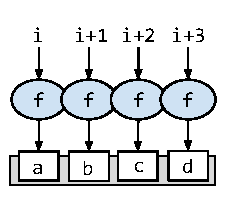
\includegraphics[width=2.6cm]{2-background/figs/Map} \\
  \texttt{\footnotesize{\textbf{Map}}} \\
\end{tabular}}
& \usebox{\MapHLL}
& \usebox{\MapPPL} \\ \hline
\vspace{-6pt} & & \\

\multirow{4}{*}{
\begin{tabular}{c}
  \vspace{-30pt} \\
  \texttt{\footnotesize{Indices}}\vspace{-6pt} \\
  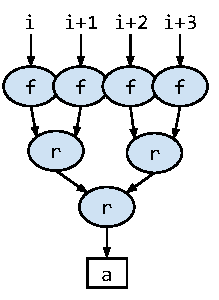
\includegraphics[width=2.6cm]{2-background/figs/Reduce} \\
  \texttt{\footnotesize{\textbf{MultiFold}}} \\
\end{tabular}\vspace{12pt}}
&
{\hspace{-6pt}\begin{tabular}{l}
\usebox{\MultiFoldHLLOne}  \\  \\
\end{tabular}}
& \usebox{\MultiFoldPPLOne} \\
\vspace{-6pt} & & \\
&
{\hspace{-6pt}\begin{tabular}{l}
\usebox{\MultiFoldHLLTwo} \\ \\ \\ \\
\end{tabular}}
& \usebox{\MultiFoldPPLTwo} \\
& & \\ \hline
\vspace{-6pt} & & \\

{\begin{tabular}{c}
  \texttt{\footnotesize{ Indices}}\vspace{-6pt} \\
  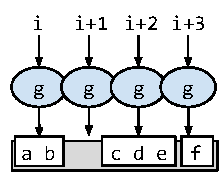
\includegraphics[width=2.6cm]{2-background/figs/FlatMap} \\
  \texttt{\footnotesize{\textbf{FlatMap}}} \\
\end{tabular}}
& \usebox{\FlatMapHLL}
& \usebox{\FlatMapPPL} \\ \hline
\vspace{-6pt} & & \\

{\begin{tabular}{c}
  \texttt{\footnotesize{  Indices}}\vspace{-6pt} \\
  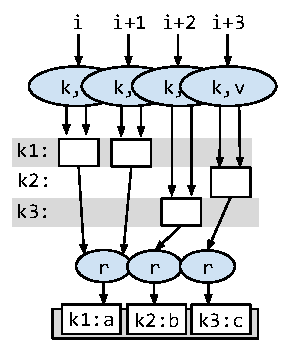
\includegraphics[width=3.2cm]{2-background/figs/HashReduce} \\
  \texttt{\footnotesize{\textbf{GroupByFold}}} \\
\end{tabular}}
& \usebox{\GroupByFoldHLL}
& \usebox{\GroupByFoldPPL} \\
\end{tabular}

\caption{\label{fig:ppl-examples}Usage examples for patterns in the PPL from various domain-specific languages.}
\end{figure*}


Figure~\ref{fig:ppl-examples} shows common examples of how users typically interact with
the patterns in PPL in various high level, domain specific languages
and how those examples are correspondingly represented in PPL. In some cases, the syntactic structure is
essentially the same except that the input domain is inferred from the shape of
the input collection. Using explicit indices in the intermediate language allows
us to model more user-facing patterns and more input access patterns with fewer internal primitives.

\emph{Map} generates a single element per index, aggregating the results into a fixed-size output collection.
Note that the value function can close over an arbitrary number of input collections, and therefore this pattern can represent classic parallel operations like \emph{map}, \emph{zip},
and \emph{zipWithIndex}.

\emph{MultiFold} is a generalization of a \emph{fold} which reduces generated values into a specified region of a (potentially) larger accumulator using an associative combine function.
The initial acummulator value $z$ is required to be an identity element of this function, and must have the same size and shape as the final output.
The main function $f$ generates an index specifying the location within the accumulator at which to reduce the generated value. We currently require the generated values to have the same arity as the full accumulator, but they may be of any size up to the size of the accumulator.
Function $f$ then converts each index into a function that consumes the specified
slice of the current accumulator and returns the new slice. If the pattern's
implementation maintains multiple partial accumulators in parallel, the combine
function $c$ reduces them into the final result.
Note that a traditional \emph{reduce} and \emph{fold} patterns are the special
case of MultiFold where every generated value is the full size of the accumulator.
The additional complexity in MultiFold is to allow the expression of tiled
parallel patterns as discussed further in Chapter~\ref{transformations}.

\emph{FlatMap} generates an arbitrary number of values per index.
These values are all concatenated into a flattened output.
As the output size can only be determined dynamically, we restrict FlatMap to
one-dimensional domains so that dynamically growing the output is easily defined.
Note that this primitive also easily expresses a \emph{filter}.

\emph{GroupByFold} reduces generated values into one of many buckets where the bucket is selected by generating a key along with each value, i.e. it is a fused version of a \emph{groupBy} followed by a \emph{fold} over each bucket.
The operation is similar to \emph{MultiFold} except that the key-space cannot be determined in advance and so the output size is unknown.
We therefore also restrict this operation to one-dimensional domains.

\begin{figure}
\centering
\begin{lstlisting}[language=Scala]
//data to be clustered, size n x d
val points: Array[Array[Float]] = ...

// current centroids, size k x d
val centroids: Array[Array[Float]] = ...

// Assign each point to the closest centroid by grouping
val groupedPoints = points.groupBy { pt1 =>
  // Assign current point to the closest centroid
  val minDistWithIndex = centroids.map { pt2 =>
    pt1.zip(pt2).map { case (a,b) => square(a - b) }.sum
  }.zipWithIndex.minBy(p => p._1)
  minDistWithIndex._2
}

// Average of points assigned to each centroid
val newCentroids = groupedPoints.map { case (k,v) =>
  v.reduce { (a,b) =>
    a.zip(b).map { case (x,y) => x + y }
  }.map { e => e / v.length }
}.toArray
\end{lstlisting}
\caption{K-Means clustering implemented using Scala collections. In Scala, \textunderscore\texttt{1} and \textunderscore\texttt{2} refer to the first and second value contained within a tuple.}
\label{fig:kmeans}
\end{figure}

\begin{figure}\centering
\begin{lstlisting}[language=Scala]
points: Array2D[Float](n,d)    // data to be clustered
centroids: Array2D[Float](k,d) // current centroids

// Sum and number of points assigned to each centroid
(sums,counts) = multiFold(n)((k,d),k)(zeros((k,d),k)){ i =>
  pt1 = points.slice(i, *)
  // Assign current point to the closest centroid
  minDistWithIndex = fold(k)((max, -1)){ j =>
    pt2 = centroids.slice(j, *)
    dist = fold(d)(0){ p =>
      acc => acc + square(pt1(p) - pt2(p))
    }{ (a,b) => a + b }
    acc => if (acc._1 < dist) acc else (dist, j)
  }{ (a,b) => if (a._1 < b._1) a else b }

  minDistIndex = minDistWithIndex._2
  sumFunc = ((minDistIndex, 0), acc => {
    pt = points.slice(i, *)
    map(d){ j => acc(j) + pt(j) }
  })
  countFunc = (minDistIndex, acc => acc + 1)

  (sumFunc, countFunc)
}{ (a,b) => {
  pt = map(k,d){ (i,j) => a._1(i,j) + b._1(i,j) }
  count = map(k){ i => a._2(i) + b._2(i) }
  (pt, count)
} }

// Average assigned points to compute new centroids
newCentroids = map(k,d){ (i,j) =>
  sums(i,j) / counts(i)
}
\end{lstlisting}
\caption{K-Means clustering represented using the parallel patterns in Figure~\ref{fig:ppl-syntax} after fusion and code motion.}
\label{fig:kmeans-fused}
\end{figure}

To provide a further example of the usage of parallel pattern operations, we will now use them to
implement a simple k-means clustering application.
For reference, first consider $k$-means implemented using the standard Scala
collections operations, as shown in Figure~\ref{fig:kmeans}.
$k$-means consumes a set of $n$ sample points each of size $d$ and
attempts to cluster those points by finding the $k$ best cluster centroids for the samples.
This is achieved by iteratively refining the centroid values.
(We show only one iteration in Figure~\ref{fig:kmeans} for simplicity.)
First, every sample point is assigned to the closest current centroid by
computing the distance between every sample and every centroid.
Then new centroid values are computed by averaging all the samples assigned to each centroid.
This process repeats until the centroid values stop changing.

Previous work~\cite{rompf12optimizing,brown16clusters,chambers10flumejava} has shown how to stage a DSL application like $k$-means, lowering it into a parallel pattern IR similar to the one we define here, as well as how to perform multiple parallel pattern fusion automatically on the IR.
One of the most important of these optimizations is fusing patterns together, both vertically (to decrease the reuse distance between producer-consumer relationships) and horizontally (to eliminate redundant traversals over the same domain).

Figure~\ref{fig:kmeans-fused} shows the structure of $k$-means after it has been lowered into PPL and
pattern fusion rules~\cite{rompf12optimizing} have been applied.
For simplicity, we have also converted the nested arrays in the Scala example to multidimensional arrays.
This translation requires the insertion of \emph{slice} operations in certain locations, which produce a view of a subset of the underlying data.
For the remainder of this work, we will assume the existence of a parallel pattern backend
for high level DSLs of interest and always start from the parallel pattern intermediate representation.

% \section{Field Programmable Gate Arrays}
%
% While this work will not attempt to give a comprehenesive description about how
% FPGAs are used or how they work, we will provide a short background
